\chapter{Method}
\section{Radial velocity components in linear theory}
One of the goals of this project is to test the viability of using the assumptions
from linear theory and study wether it is a good physical approximation for
studying the physics of voids and filaments. The radial velocity component of
halos in filaments and voids is an analytical tool that is useful for comparing
with data from simulation for testing wether linear theory can be used to
approximate the physical behaviour of halos and galaxies observed in these objects.
\subsection{Radial velocity component for filaments}
When calculating the radial velocity component of filaments, the average filament is
approximated to be a cylindrical object. The radial component is the component of
the velocity vector $\vec{v}$ that points perpendicular to the longitudinal axis
$L$. This is illustrated in figure \ref{fig:filamentvr}. For this analysis we
will assume that the other velocity components are negligible and that the
radial component is the significant component.
\begin{figure}\label{fig:filamentvr}
    \begin{tikzpicture}
        \draw[->] (-4,0,0) -- (4,0,0) node[below right] {$L$};
        \draw[->] (0,1,0) -- (0,0.5,0) node[below right] {$v_r$};
        \draw[->] (0,-1,0) -- (0,-0.5,0) node[below right] {$v_r$};
        \node (A) [draw, cylinder, shape aspect=1.8, minimum height=50mm, minimum width=20mm] {};
    \end{tikzpicture}
    \caption{Illustration of a cylindrical filament with longitudinal axis $L$ and radial velocity component $v_r$.}
\end{figure}
in linear theory can be written as
\begin{equation}\label{eq:lincont}
    \frac{d\delta}{dt}+\frac{1}{a}\nabla\cdot\vec{v}=0.
\end{equation}
 The continuity equation In linear theory one can write
 $\frac{d\delta}{dt}=Hf\delta$ \cite[p.~347]{schneider2006extragalactic}, where $f$ is the growth factor
defined in equation \ref{eq:growthfac}. Substituing this into equation
\ref{eq:lincont} one will get
\begin{equation}\label{eq:templineq}
    \nabla\cdot\vec{v}=-Hfa\delta.
\end{equation}
Assuming cylindrical coordinates we can replace the
divergence
\begin{equation}
    \nabla\cdot\vec{v}=\frac{1}{r}\frac{\partial}{\partial r}(rv_r)+\frac{1}{r}\frac{\partial v_\phi}{\partial \phi} +\frac{\partial v_L}{\partial L}.
\end{equation}
Assuming that the radial component $v_r$ gives the significant contribution and
the two other are negligible, by inserting into equation \ref{eq:templineq} on
will get
\begin{equation}
    \frac{1}{r}\frac{\partial}{\partial r}(rv_r)=-Hfa\delta.
\end{equation}
Multiplying both sides by $r$ and integrating one will be left with
\begin{equation}
    v_r=-\frac{1}{r}Hfa\int_0^r\delta(r^\prime) r^\prime dr^\prime.
\end{equation}
By defining the average mass density contrast for filaments $\Delta_f(r)$
as
\begin{equation}\label{eq:contrastfil}
    \Delta_f(r)=\frac{2}{r^2}\int_0^r\delta(r^\prime) r^\prime dr^\prime,
\end{equation}
one can write the radial velocity component for a halo in a filament as
\begin{equation}\label{vrfilament}
    v_r(r) = -\frac{1}{2}Hfar\Delta_f(r).
\end{equation}
\subsection{Radial velocity component for voids}
The radial velocity component for voids is similar to the one for filaments
except that for voids one assumes a spherical coordinate system. This assumption
is based on the notion that the average void should have a spherical shape with,
on average, no prefferred direction for overdensities on the rim and
thereby having a spherical density profile. Since objects cluster towards larger
densities, approximating the velocity of halos and galaxies around
voids to be dominated by the radial component, moving straight away from the
underdensity in the center of the void one can argue that the radial velocity
should be the dominating component. This is illustrated in figure \ref{fig:filamentvr}.
\begin{figure}\label{fig:filamentvr}
    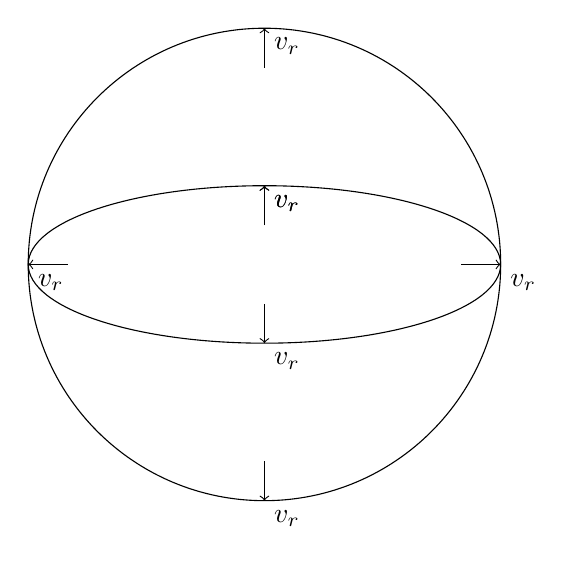
\begin{tikzpicture}
        \draw[->] (0,0.5,0) -- (0,1,0) node[below right] {$v_r$};
        \draw[->] (0,-0.5,0) -- (0,-1,0) node[below right] {$v_r$};
        \draw[->] (0,0.5,0) -- (0,1,0) node[below right] {$v_r$};
        \draw[->] (2.5,0,0) -- (3,0,0) node[below right] {$v_r$};
        \draw[->] (-2.5,0,0) -- (-3,0,0) node[below right] {$v_r$};
        \draw[->] (0,2.5,0) -- (0,3,0) node[below right] {$v_r$};
        \draw[->] (0,-2.5,0) -- (0,-3,0) node[below right] {$v_r$};
        \draw (0,0) circle (3cm);
        \draw (0,0) ellipse (3cm and 1cm);
    \end{tikzpicture}
    \caption{Illustration of a spherical void with radial velocity pointing outwards from the center of the void.}
\end{figure}
The derivation for the radial velocity component is the same for voids as for
filaments up until equation \ref{eq:templineq}. The difference for voids is that
the divergence now has to be calculated in spherical coordinates given by
\begin{equation}
    \nabla\cdot \vec{v}=\frac{1}{r^2}\frac{\partial}{\partial r}(r^2v_r)
                       +\frac{1}{r\mathrm{sin}\theta}\frac{\partial}{\partial r}(\mathrm{sin}\theta v_\theta)
                       +\frac{1}{r\mathrm{sin}\theta}\frac{\partial}{\partial r}(\phi v_\phi).
\end{equation}
As for filaments only the radial component is assumed to be non-negligible
giving
\begin{equation}
    \frac{1}{r^2}\frac{\partial(r^2v_r)}{\partial r}=-Hfa\delta.
\end{equation}
Multiplying by $r^2$ and integrating one will get
\begin{equation}
    v_r = -\frac{1}{r^2}Hfa\int_0^r r\prime^2\delta(r^\prime)dr^\prime.
\end{equation}
As for filaments a average mass density contrast for voids is defined as
\begin{equation}\label{eq:contrastvoid}
    \Delta_v(r)=\frac{1}{r^3}\int_0^r r\prime^2\delta(r^\prime)dr^\prime,
\end{equation}
which will give an expression for the radial velocity for voids
\begin{equation}\label{eq:vrvoid}
    v_r(r)=-Hfar\Delta_v(r).
\end{equation}